%%% 関西大学 総合情報学部 松下ゼミ 進捗報告 TeXテンプレート Ver 1.1 (2011/12/04) %%%
\documentclass{matsushita-zemi}
\usepackage[dvipdfmx]{graphicx}
\usepackage{comment}
\usepackage{ascmac}
\graphicspath{{./fig/}}

%%% タイトル (長くなる場合は¥¥で適宜改行すること)%%%
\title{Elucignage: 効率的な情報アクセスのための動向情報可視化インタフェース}

%%% 氏名 (姓・名の間は半角スペース) %%%
\author{内藤 峻}

\begin{document}
\maketitle

%%% 以下、本文 %%%
%\section*{概要}
%\label{abstract}
%ネットワーク上には多様な種類の情報が存在しており、それらをユーザの要求に応じて適応的にまとめ上げる技術が渇望されている。その一つとして、テキストなどの言語情報と統計データなどの数値情報の相補的な利用に関する研究が行われている。その一環として、本研究では言語情報と数値情報が密接な関係にある株価などの動向情報に着目しそれらを統一的な枠組みで可視化する手法を提案する。株価などの統計情報の場合、その正確な値を知るには数値情報が適切であるのに対して、変動の大局的な理解や背景となる事象の把握には言語情報が適している。そこで、これらを一つのグラフ上に提示し、その情報源に対話的にアクセスできるようにする。

\section{はじめに}
\label{background}
%電子化が普及している話
%それらの情報を利用して意思決定や問題解決に役立てられている話
%しかし、情報は膨大になっている、時間にともなって更に増加を続けている話
%既存の検索技術ではユーザの要求に答えることができない
%それらをまとめる技術が求められている話
%しかし、情報には様々な種類がある話
%以上のことを解決するためのコミュニティがある話
%動向情報の話
%本提案では数値情報(統計データ)と言語情報(新聞記事)に着目した話

近年、コンピュータの処理能力の向上やネットワークの発達に伴い、電子化された情報は増加の一途を辿っている。\begin{comment}
電子化された情報は場所を取らず、劣化もせず、複製も容易であり、どこからでもアクセスできる、といった利点がある。新聞記事や統計データ、書籍など、様々な情報が電子化されている。これらの膨大な情報は単なるアーカイブとしての役割に留まらず、意思決定や問題解決に役立てるために有益な情報や知識を得るためのリソースとして期待されている。
\end{comment}
それに伴い、これらの情報を利用して意思決定や問題解決に役立てる試みがなされている。しかし、蓄積された情報は膨大であるうえ、時間の経過に伴って更に増加を続けている。そのため、“情報の在処を見つける”ことを主眼とした検索技術ではユーザの要求に十分に応えることができず、ユーザの関心や興味に合致する情報に直感的かつ簡便にアクセスするための技術、言うなれば“情報の理解”を助ける技術が渇望されている。このような背景の下、新聞記事テキストや統計データといった異なる形式の情報を相補的に用いて編纂し、ユーザの情報アクセス行為を容易にする技術(情報編纂技術)の実現を目指している\cite{information_compilation}\cite{InformationcompiledStudyGroup}。ネットワーク上にはテキストだけでなく、音声や画像、動画など様々な形式の情報が存在している。情報編纂技術が目指すのは、これらの情報をユーザの興味や関心に基づいて適応的に再構成し一纏まりの情報として提示すると共に、それをトリガとしたインタラクティブな情報アクセスを可能にすることである。このような要求に応える技術の一つとして、松下らは動向情報を対象とし、それらを要約・可視化する技術の研究を行っている\cite{STEND}。

動向情報とは、ある商品の価格や売上高、台風の進行状況や被害の経過、内閣や政党の支持率の推移など幾つかの統計量や出来事に関する時系列データを基にして、ある観点の下でその変化を通時的に捉えて纏めあげたものである。このような動向情報は単なる一次元の時系列情報ではなく、製品のシェアのように複数の企業が関係したり、地域ごとの土地価格の変動のように空間的な広がりを持ったりするなど、複数主体や空間軸を含んだ多次元情報である。

松下らが目指しているのは、動向情報に対するユーザの関心・質問に、簡潔で平易な文章や可視化表現(グラフなど)を組み合わせて応答するマルチモーダル質問応答システムの実現であり、そのための要約と可視化である。本稿ではその手始めとして統計データなどの数値情報と新聞記事などの言語情報を相補的に用いて編纂し、ユーザの情報アクセス行為を容易にする技術の実現をめざす。

%松下らが目指しているのは、例えば「去年から今年にかけてガソリンの価格ってどう動いていますか?」や「作シーズンの大リーグのホームラン競争ってどんな経過だったのですか?」のような、動向情報に対するユーザの関心・質問に、簡潔で平易な文章や可視化表現(グラフなど)を組み合わせて応答するマルチモーダル質問応答システムの実現であり、そのための要約と可視化である。本稿ではその手始めとして統計データ等の数値情報と新聞記事等の言語情報を相補的に用いて編纂し、ユーザの情報アクセス行為を容易にする技術の実現をめざす。

%近年、様々な情報が電子化されネットワーク上に蓄積されている。それに伴い、これらの情報を利用して意思決定や問題解決に役立てる試みがなされている。しかし、蓄積された情報は膨大であるうえ、時間の経過に伴って更に増加を続けている。そのため、"情報の在処を見つける"ことを主眼とした検索技術ではユーザの要求に十分に応えることができず、ユーザの関心や興味に合致する情報に直感的かつ簡便にアクセスするための技術、言うなれば"情報の理解   "を助ける技術が渇望されている。

%近年、コンピュータの処理能力の向上やネットワークの発達に伴い、電子化される情報は増加の一途を辿っている。電子化された情報は場所を取らず、劣化もしない、複製も容易であり、どこからでもアクセスできる、といった利点がある。新聞記事や統計データ、書籍など、様々な情報が電子化されている。これらの膨大な情報は単なるアーカイブとしての役割に留まらず、意思決定や問題解決に役立てるために有益な情報や知識を得るためのリソースとして期待されている。
%近年、様々な情報が電子化されネットワーク上に蓄積されている。それに伴い、これらの情報を利用して意思決定や問題解決に役立てる試みがなされている。しかし、蓄積された情報は膨大であるうえ、時間の経過に伴って更に増加を続けている。そのため、"情報の在処を見つける"ことを主眼とした検索技術ではユーザの要求に十分に応えることができず、ユーザの関心や興味に合致する情報に直感的かつ簡便にアクセスするための技術、言うなれば"情報の理解   "を助ける技術が渇望されている。
%このような要求に答える技術のひとつとして、本提案では統計データ等の数値情報と新聞記事等の言語情報を相補的に用いて編纂し、ユーザの情報アクセス行為を容易にする技術の実現をめざす。

%ネットワーク上にはテキストや統計データ、音声、画像動画など様々な種類の情報が存在している。
%将来的にはそれらの情報全てを対象とし、状況や目的に応じて取捨選択やモード変換を行い、適切な形態で組み合わせてユーザに提供することが望まれるが、現在の技術レベルではその実現は容易ではない。本研究では、時間的変動を伴う統計データ(時系列数値情報)とそれに関連する記事(言語情報)を対象とし、ユーザがそれらの情報にアクセスしたり、その概要を把握したりする際の支援となる可視化手法について議論する。

本稿では、まず、動向情報の可視化に関する先行研究を挙げ、本研究に有用な手法について取り上げる。次に、本研究の提案システムのデザイン指針を示し、その後、卒論に向けた進捗状況と今後の展望を報告する。

\section{先行研究}
\label{relatedworks} 
%動向情報を可視化する研究として、山本らの可視化システム\cite{Tagged_corpus}や小泉らの被験者実験\cite{interconversion}、松下らのSTEND\cite{STEND}、高間らの地震情報可視化システム\cite{SpaceTrendInformation}、太田らの可視化手法\cite{numerical_features}などがある。
本章では動向情報を可視化する研究について報告する。

山本らは、
\begin{comment}
近年、電子化された情報の増加に伴い、
\end{comment}
ユーザの関心や興味に合致する情報に直感的かつ簡便にアクセスするための技術の一つとして、動向情報の変化とその変化要因とを視覚的に表示するシステムを開発している\cite{Tagged_corpus}。システムは、内閣支持率に関連する新聞記事を入力することにより、内閣支持率の推移グラフを出力し、ユーザの興味と見やすさを考慮し、内閣支持率の変化の大きい部分などにその変化の根拠となる要因をグラフ上に配置している。
\begin{figure}[tb]
  \begin{center}
   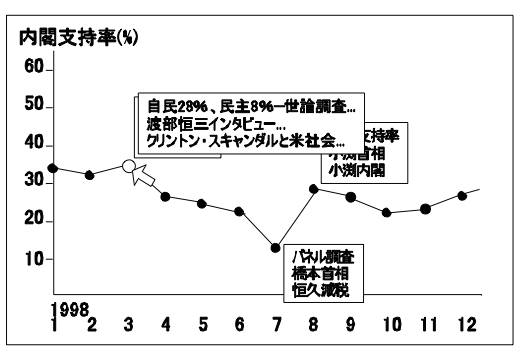
\includegraphics[width=8cm,bb=0 0 521 356]{tagu.PNG}
  \end{center}
 \caption{山本らのシステムの出力例}
 \label{system}
\end{figure}
%山本らは、記事中に存在するある時点の変化についての定性的な記述や、原因や影響に関する記述を注釈としてグラフに与える方法を提案している\cite{Tagged_corpus}。例えば内閣支持率の場合、過去のある時点の支持率と関係が強い出来事を注釈することで、どのような事件が支持率に影響を与えたかをユーザが把握・判断できるようにしている。値の変化の大きな点、減少から増加に転じる極小点など、利用者が関心を持ちそうな点に選択的に情報を付与することによって視認性の向上を測り、ユーザにとって分かりやすい情報提示を目指している。

%この方法は本稿の提案方法と問題意識が近く、特に情報提示に関しては参考になる点も多い。しかし、その情報提示がユーザとのインタラクションにおいてどのように作用し適応していくかについては、現状ではあまり深く検討されていない。本提案はユーザのインタラクションに基づく適応的情報提示に大きな関心があり、この点でこれらの方法と方向性が異なる。

%先生に確認する

小泉らはグラフを説明した文章の収集とその文章の適切さを目的として、
\begin{comment}
言語情報と統計グラフの相互変換技術について研究している\cite{interconversion}。その一つとして、被験者実験を通じて、
\end{comment}
人がグラフを文章に符号化する際に使用する語彙や文章構造について調べている\cite{interconversion}。その結果、文章の構造を語彙の出現頻度によっておおよそ分類可能であることを示している。分類は5パターンある。
\begin{enumerate}
 \item グラフを左から右に向かって説明する
 \item 全体的な形で説明する
 \item 左から右に向かって説明した後に全体的な形を説明する
 \item 全体的な形で説明した後に左から右に向かって説明する
 \item その他
\end{enumerate}
%この分類は、新聞記事に適応でき、分類語を用いることによって文章からどのような内容が述べられているかを把握することができる。そのため、本研究のElucignageシステムの矢印アイコンの選定に有効であると考える。分類語を用いた自然言語処理を行うことによって、分類語に近い数値情報を取得し、それに応じたアイコンを選定することが可能であると考える。以下にこの研究を通して行われた研究を報告する。

松下らは、グラフ概形を示唆するシステムSTENDを提案している\cite{STEND}。STENDは時系列数値情報を扱わず、新聞記事のテキストデータのみから取得可能な数値情報と定性情報に着目してグラフ描画を試みたものである (図\ref{STEND}) 。テキスト中の「昨年10月より約40%の下落になっている」「前年同月に比べて5ドル上昇した」等の比較表現や「安定傾向にあった」「10月をピークに下落している」等の定性表現から情報を抽出している。情報提示では、統計グラフを用いず数種類の点や短形、形状の異なる幾つかの矢印記号を組み合わせることでその代替を試みている。
\begin{figure}[tb]
  \begin{center}
   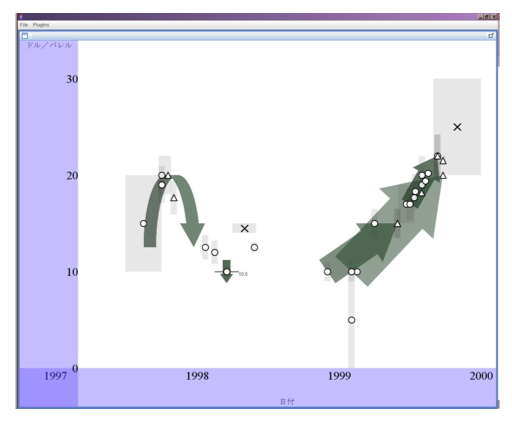
\includegraphics[width=8cm,bb=0 0 512 422]{STEND.PNG}
  \end{center}
 \caption{STENDの描画例}
 \label{STEND}
\end{figure}

高間らは空間的な動向情報を含んだ可視化システムについて提案している\cite{SpaceTrendInformation}。
動向情報の可視化の対象として選択されているのは、時間情報と数値情報がほとんどである。この研究ではこれらの時系列情報に空間情報を加えた地震情報を対象としている。これは本研究のねらいである多様な種類の情報を編纂するという点で有望であると思われる。
%Elucignageシステムの展望として、動向情報だけでなく、空間情報もシステムの機能として検討していきたい。
%地震や台風などは時間的な動向情報だけでなく空間的な動向情報を含んでおり、両者を考慮した可視化が必要となる。提案システムでは地図もしくはグラフと検索クエリを入力するフォーム、それに対応する新聞記事を一画面に提示している。複数の地震について同じ空間へ描画することを可能にしている。


太田らは文書中の数値的特徴を用いた情報可視化につて述べている\cite{numerical_features}。
この論文では、記事から抽出されたデータの特徴を基に適切なグラフの種類を決定し、グラフの作成を行う手法について述べている。折れ線グラフは時間経過による数量の変化を視覚的に表示するときに適していることや、棒グラフは数量の比較を視覚的に表示するときに適しているなど、各グラフの特徴について詳しく述べられている。これは本研究のねらいである異なる形式の情報を相補的に用いて編纂し、ユーザの情報アクセス行為を容易にする技術(情報編纂技術)の実現において有用であると考えられる。
%Elucignageシステムが将来的に状況や目的に応じてやモード変換を行ううえで

\section{デザイン指針}
%目的をどのように達成するのかという話
%どのような機能が必要なのか?何故必要なのか?
%シナリオに基づいた話
%必要な機能な整理
%シナリオを載っけるのもあり
%言語情報と数値情報を扱う話
%それらをどのように見せるか、どのようなインタラクションを想定するのかという話
%変化の実験の論文を引用
%統計情報等の数値情報は正確である。
%変わって、言語情報はあいまいであるものの、その時点の背景等を理解することができる。
%本研究では、数値情報には統計DBを、言語情報には新聞記事を用いて、ユーザの効率的なアクセスを促すシステムを提案する。
%ユーザの効率的なアクセスを支援するためにはユーザのふるまいを想定をする必要がある。
%ユーザはグラフを見て、そのときの変化における要因や背景を知りたいと思う。そこで、本提案ではユーザの興味や関心を想定したインタラクションを考える。
%ユーザはグラフの変曲点になる部分に興味を持つ。
%また、そこで、要因と背景を知りたいと思う。
%以下の様なシナリオを想定している。
本研究では、既存の検索技術を用いてユーザの意思決定や問題解決に役立つシナリオを想定し、システムに必要な機能を整理する。以下に、複数あるシナリオの中からガソリンに関係するシナリオを示す。
\begin{itembox}[l]{シナリオ1}
工場を経営しているAさんは最近、自社で扱っているガソリンの価格が上昇していることを知り、不安に思い始めた。そこで、最近のガソリンの価格を調べることにした。すると、ガソリンの価格はある程度上下するものだとわかった。しかし、ある程度上下するものの価格は上昇傾向にあった。何故、上昇傾向にあるのか調べてみると、背景に外国情勢が絡んでいた。一つはウクライナ情勢である。産油国のロシアから欧州への原油供給が止まる可能性が取りざたされていた。さらに、同じく産油国のイラクでも6月から武装組織が活動を活発化させ、原油の供給が脅かされていることや円ドル相場が2013年初頭と比べ10\%ほど円安になり、輸入コストが増大していること、さらには、経営の厳しさが増す国内の石油元売各社やガソリンスタンドが、収支改善のために原料の上昇分を店頭価格に反映させ始めたとの指摘もあることがわかった。念のため、円ドル相場を調べてみると、2013年初頭と比べて円安になっていた。調べていくうちに、もしかすると「夏にガソリンの価格が上がるのではないか」と考え、過去の3年分のデータを調べることにした。すると、夏と冬をピークに価格が上下することがわかった。また、2008年に価格が急上昇しているのをみて、何故こうなったのか原因を調べることにした。調べてみると、アメリカの金融危機が原因だとわかった。Aさんは不安を解消することができ、安心してガソリンを購入しようと決意した。
\end{itembox}

\begin{itembox}[l]{シナリオ2}
運送業者の経営をしているCさんは2013年3月、最近の自社の売上が低下していることに頭を悩ましていた。そこで、何故売上が低下しているのか調べてみることにした。すると、ガソリンの購入額が上がっている事に気づいた。Cさんは何故こんなにもガソリンにお金がかかっているのか調べることにした。最近一ヶ月のガソリンの価格を調べてみると、確かに上昇傾向にあった。いつから上昇傾向にあるのか知りたいと思い、もう少しさかのぼって調べてみた。すると、3ヶ月前から上がっていることがわかった。そこで、何故こんなにも上がっているのか疑問に思い、理由を調べることにした。すると、薄水色線のドバイFOB価格(右軸\$/B)が、105ドルから113まで値上がりしたのと円安で、TOCOM東京ドバイ価格(橙色)も高騰したためだとわかった。そして、何故ドバイ原油価格が上昇しているのか調べてみると、近年、中国、インド、インドネシアなどアジア諸国での需要の拡大が関係していることがわかった。Cさんは自社の売上が低下した原因を知ることができ、しばらくこの調子で経営することに決めた。
\end{itembox}

\begin{itembox}[l]{シナリオ3}
貨物輸送の経営者のBさんは最近(2014年8月4日)、軽油の価格が下がってきていることを知り、この減少がいつまで続くのか、そして、買い時がいつ頃なのか知りたいと思い始めた。そこで、最近1ヶ月の軽油の価格を調べることにした。すると、徐々にではあるが減少していることがわかった。しかし、この情報だけではこれからの価格を推測することができなかったので、最近一年間の価格を調べることにした。すると、先月をピークに下がってきていることがわかった。次に、毎年このようなピークがあるのか調べるために、2年前〜1年前の価格を調べることにした。すると、去年の3月にピークがあることがわかった。また、去年の今頃から現在に至るまで上昇傾向にあることがわかった。そこで、何故軽油が去年の7月から上昇しているのか気になり、調べてみることにした。すると、軽油は原油価格によって変動するものであり、アメリカの株価の動向、中東情勢の政治的な動き、ヨーロッパの景気動向、特に金融不安の解消、さらには発展途上国の状況によって影響されるものだとわかった。また、ドルベースの原油価格の上昇と円安が複合的に作用したからだということもわかった。読み進めると、米国のエネルギー輸出は徐々に許可される方向にあり、それにともなって原油価格も安定してくると考えられていることがわかった。そこで、Bさんは現在の軽油の価格がまだ下がりそうだと考え、もう少し待つことにした。
\end{itembox}

以上のシナリオから必要な機能のリストを以下に示す。
\begin{description}
 \item[検索を可能にする]\mbox{}\\ 
 シナリオ1、2、3に共通して見られるのが複数の統計情報をまたいで分析していることである。シナリオ1ではガソリンの価格から円ドル相場へ、シナリオ2ではガソリンの価格からドバイ原油価格へ、シナリオ3では軽油の価格から原油の価格へと見たい統計情報が変わっている。
 \item[グラフの表示領域の変更を可能にする]\mbox{}\\
 シナリオ1の「過去の3年分のデータを調べることにした」やシナリオ2の「もう少しさかのぼって調べてみた」、シナリオ3の「2年前〜1年前の価格を調べることにした」という記述からグラフを拡大、縮小、表示領域を変更可能にする機能が必要だと考えられる。
 \item[理由や背景を参照できるインタラクションを付与する]\mbox{}\\
 シナリオ1の「何故、上昇傾向にあるのか調べることにした」やシナリオ2の「何故売上が低下しているのか調べてみることにした」や「何故こんなにも上がっているのか疑問に思い、理由を調べることにした」、シナリオ3の「何故軽油が去年の7月から上昇しているのか気になり、調べてみることにした」という記述から、理由や背景を参照できるインタラクションが必要であることが考えられる。また、インタラクションを付与するためのトリガが必要であることが考えられる。
 \item[動向情報を予測する]\mbox{}\\
 シナリオ1の「もしかすると夏にガソリンが上がるのではないか」やシナリオ3の「買い時がいつ頃なのか知りたい」という要求から動向情報の予測を望んでいることが考えられる。
 \item[最低値と最高値、平均を表示する]\mbox{}\\
 シナリオ1と3に「ピーク」という記述がいくつかされていることから、ユーザはその期間の最低値と最高値が知りたいのではないかと考えられる。また、シナリオ3のような「買い時がいつ頃なのか知りたい」という予想を立てる際にはその期間の平均値を知ることができればユーザにとって嬉しいと思われる。
\end{description}

%以上のシナリオから必要な機能を選定する。まず、シナリオ1、2、3に共通して見られるのが複数の統計情報をまたいで分析していることである。シナリオ1ではガソリンの価格から円ドル相場へ、シナリオ2ではガソリンの価格からドバイ原油価格へ、シナリオ3では軽油の価格から原油の価格に、と見たい情報が変わっている。また、シナリオ1の「過去の3年分のデータを調べることにした」やシナリオ2の「もう少しさかのぼって調べてみた」、シナリオ3の「2前~1年前の価格を調べることにした」という記述からグラフを拡大、縮小、表示領域を変更可能にする機能が必要だと考えられる。次に、シナリオ1の「何故、上昇傾向にあるのか調べることにした」やシナリオ2の「何故売上が低下しているのか調べてみることにした」や「何故こんなにも上がっているのか疑問に思い、理由を調べることにした」、シナリオ3の「何故軽油が去年の7月から上昇しているのか気になり、調べてみることにした」などの記述から、理由や背景を参照できるインタラクションが必要であることが考えられる。最後に、先ほど述べたインタラクションを付与するためのトリガーが必要であることが考えられる。

%以上のシナリオを踏まえて、動向情報に対するユーザの関心(e.g.,最近数ヶ月のガソリン価格の変化、ここ数年の携帯電話加入者数の推移)に応じて数値情報を統計グラフとして描画し、その上に各々の時点の情報をその内容に応じてアイコン形式で重ねて提示する方法を提案する。このアイコンはテキスト情報へのポインタの役割も兼ねている。そのため、ユーザは描画されたグラフ自体を、自分の知りたい情報の外観(要約)として利用出来るだけでなく、興味を持った箇所についてどのようなことが述べられているかを背景となっている文書群にアクセスすることで確認できる。また、そこからグラフの該当箇所へジャンプする機能を付与する。これにより、注目した記事がどのような状況下で記述されたものであるかをグラフにアクセスすることで確認できる。

\section{Elucignageプロトタイプシステム}
\subsection{概要}
%書き直し、もう少し詳しく述べられるはず
ユーザは統計グラフの外観を理解するだけでなく、興味を持った箇所についてどのようなことが述べられているかをその要因となる記事にアクセスすることで参照できる。そのため、ユーザの関心がある動向情報を時系列数値情報を用いて統計グラフとして描画し、そのグラフの要因となる記事をその内容に適したアイコンの形式で提示する方法を採用する。このアイコンは要因となる記事のアクセスを可能にする。また、記事の一部を画面の一部に表示し、そこからグラフのどの部分に該当しているかを示す機能を備える。これにより、要因となる記事がグラフのどの部分で記述されたものであるかを確認できる\cite{Elucignage-jsai}\cite{Elucignage}。
\subsection{進捗状況}
%現段階の実装に関して述べる。
%検索ボックス
%記事リストパネル
%グラフパネル
%コントロールパネル
%使ったデータの図を貼る
試作したElucignageプロトタイプの外観を図\ref{Elucignage}に示す。システムはHTML、CSS、javascriptを用いて実装した。JavaScriptのライブラリはjquery-1.6.2.jsとD3.jsを用いている。現在は外観とグラフの描画、新聞記事を提示する機能を実装したところである。
このプロトタイプは、記事リストパネルに新聞記事を表示するボタン (図\ref{Elucignage}左上画面) 、記事のスニペットを表示する記事リストパネル (図\ref{Elucignage}左下画面) 、グラフとそれに関連する記事へのポインタであるアイコンを表示するグラフパネル (図\ref{Elucignage}右上画面) から構成される。

ユーザがボタンをクリックすると、記事リストパネルに記事の一覧がスニペットを伴って表示される。スニペットはユーザに元記事を参照する価値があるかどうかの判断材料として提示されるものである。グラフパネルにはシステム起動時にグラフとアイコンが表示される。

現在の実装はボタンをクリックすると新聞記事の一部を提示するようになっている。また、スニペットは以下に示すxml形式のファイルからTEXTタグに含まれている本文を表示させている。グラフはD3.jsを用いて描画している。
\begin{verbatim}
<?xml version="1.0" encoding="Shift_JIS"?>
<DOC>
<DOCNO>980214080</DOCNO>
<SECTION>経済</SECTION>
<AE>有</AE>
<WORDS>635</WORDS>
<HEADLINE>「イラク危機、原油の需給バランスに影響ない」−−通産省は静観の構え</HEADLINE>
<TEXT>
 米国とイラクの緊張が続いているが、通産省は今のところ「米国がイラク攻撃に踏み切っても、影響がイラク原油・・・
</TEXT>
</DOC>
\end{verbatim}

ユーザがアイコンをクリックすると記事のスニペットの文字が大きくなる (図\ref{Elucignage_click})。これはユーザがグラフ上のある点に興味や関心を持った際にグラフから新聞記事へ視線を誘導するためのものである。

\begin{figure}[tb]
  \begin{center}
   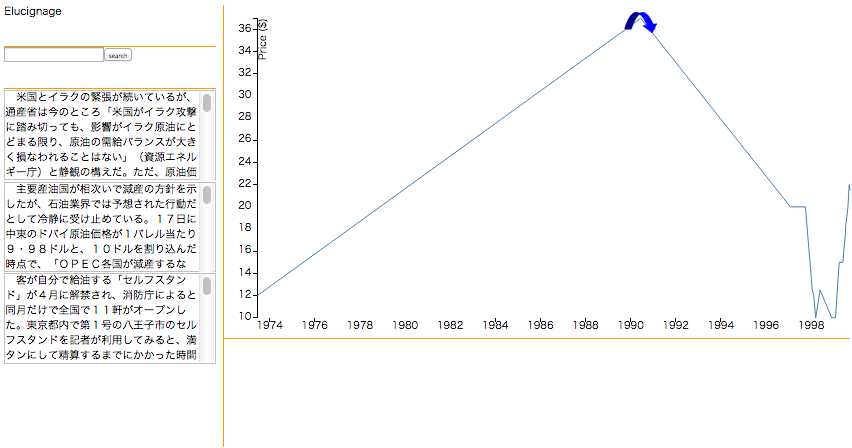
\includegraphics[width=8cm,bb=0 0 852 448]{Elucignageprototype.png}
  \end{center}
 \caption{Elucignageのスナップショット}
 \label{Elucignage}
\end{figure}
\begin{figure}[tb]
  \begin{center}
   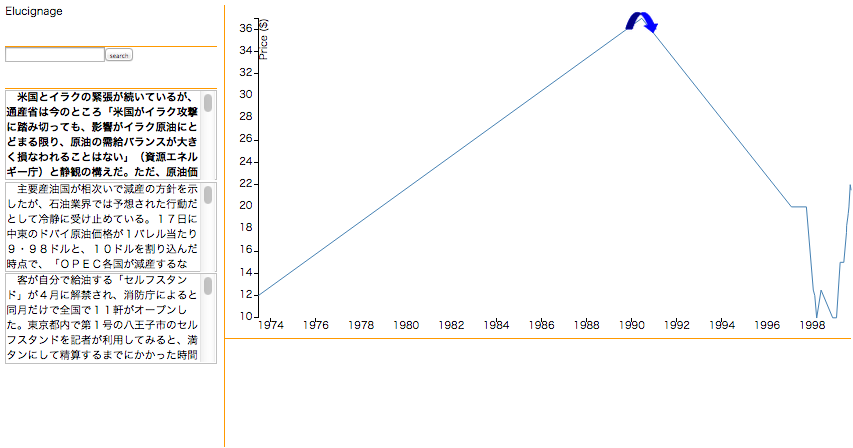
\includegraphics[width=8cm,bb=0 0 853 448]{Elucignage_click.png}
  \end{center}
 \caption{Elucignageのスナップショット(アイコンをクリックしたとき)}
 \label{Elucignage_click}
\end{figure}

\subsection{今後の展望}
%ボタンを検索可能な検索ボックスにする
%スニペットには指示的な要約を用いる
%関連記事の同定や選択、スニペットの生成の自動化
%コントロールパネル(オーバービューエリアを含めた)を実装する
%アイコンの自動生成
この節ではこれから実装する予定である機能を示す。まず、グラフの描画範囲を変更することができるコントロールパネルを実装する。次に、検索を可能にする。ボタンを検索ボックスにし、統計情報の一部を入力すると、グラフパネルにグラフとアイコンが表示されるようにする。また、同時に記事リストパネルに関連する記事の一覧がスニペットを伴って表示されるようにする。その後は、関連記事の同定や選択、スニペット、アイコンの生成の自動化を考えていく。


\section{おわりに}
本稿では、ユーザの興味や関心への効率的なアクセスを可能にする可視化インタフェースについて考察した。
%本稿では、動向情報の可視化手法について考察した。先行研究として山本らの可視化システムや小泉らの被験者実験、松下らのSTEND、高間らの地震情報可視化システム、太田らの可視化手法を報告した。続いて、本研究のシステムのデザイン指針を説明し、卒業研究への展望を示した。

%%% 参考文献 %%%
\bibliographystyle{ipsjsort}
\bibliography{reference}

\end{document}